\documentclass[letterpaper,10pt]{article}

\usepackage[english]{babel}
\usepackage[utf8]{inputenc}
\usepackage{amsmath}
\usepackage{graphicx}
\usepackage[colorinlistoftodos]{todonotes}
\usepackage[top=0.5in, bottom=0.5in, left=0.9in, right=0.9in]{geometry}
\usepackage[small]{titlesec}

\newcommand{\bes}{\begin{equation*}}
\newcommand{\ben}[1]{\begin{equation}\label{#1}}
\newcommand{\ees}{\end{equation*}}
\newcommand{\be}{\begin{equation}}
\newcommand{\ee}{\end{equation}}

\titlespacing{\section}{0pt}{\parskip}{-\parskip}

\begin{document}

\begin{flushright}
{\Large Josh Bevan - Final Project (Mixed vs LSQ) - CS555}
\end{flushright}
\vskip -0.1in
\hrule
\vskip 0.4in

\section*{Description of Problem}
The problem under consideration is the Poisson problem:
\bes -\nabla \cdot \nabla u = f \ees
with a constant one $f$ over the domain and zero Dirichlet boundary conditions. The domain is an L-shape extending from -1 to 1 in both axes. Figure 1 shows the domain and an example FEM solution. One issue readily apparent from the example solution is the singularity at the elbow of the domain, where the contours are very closely spaced.

The problem was solved in first order form:
\bes q = \nabla u\ees
\bes \nabla \cdot q = f \ees

so that the problem has the form $Lu = f$, with:
\bes L = \begin{bmatrix}I & -\nabla\\ -\nabla \cdot & 0\\ \nabla\times & 0\end{bmatrix}\ees

In order to examine convergence/performance behavior of Dolfin's solution of this problem two approaches are considered: mixed and least-squares finite element methods. Both $p$ and $h$ refinement are considered for both methods. For a desired accuracy the best combination of each will be determined that leads to the shortest runtime.

\begin{figure}[!htb]
\centering
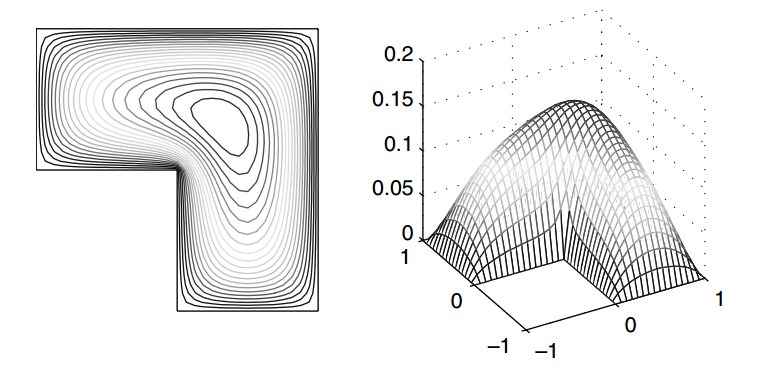
\includegraphics[width=1 \linewidth]{prob.PNG}
\caption{Domain under consideration and example FEM solution. \newline \small [1] https://relate.cs.illinois.edu/course/cs555-s17/file-version/ e7705789e10f2d32e20ca9afcfe5319e64705316/book/poissonequation.pdf}
\end{figure}
\newpage
\section*{Experimental Setup}
In order to determine the accuracy of the numerical solution, it must be compared against some standard. While an analytical solution is not available across the full domain, a analytical solution that is valid in the direct neighborhood of the elbow is available from [1]:

\bes u(r,\theta) = r^{2/3} \, sin((2\theta + \pi)/3).\ees

Therefore, each numerical solution can be compared to this analytical solution and a error norm can be calculated. However because the analytical solution is true only in the direct neighborhood a ``selector'' function was used to weight both the numerical and analytical solutions, so that their behavior only in the direct neighborhood has any effect on the error norm:

\bes w(x,y) = exp(-1(\frac{(x-0)^2}{2*\sigma_x^2}+\frac{(y-0)^2}{2\sigma_y^2})) \ees
\bes weighted \;error = |u_h*w-u_e*w|_{L^2}\ees

In practice it was found $\sigma=0.005$ was an appropriate cutoff radius for the Gaussian weighting function. This value was chosen to balance including as much of the solution as possible, while still only selecting a neighborhood for which the analytical solution was still valid.

The mixed finite element method used Lagrange and Brezzi-Douglas-Marini spaces. This combination was chosen based on suggestions from Dolfin demos and examples.

A series of solutions were then calculated and the timing and weighted errors were recorded for four levels of h-refinement and 3-levels of p-refinement for each finite element method.\\

\section*{Results}
Qualitatively, solutions from both mixed and LSQ methods were not adequately converged for the base h-refinement, while for all other h and p refinement level combinations, the solution closely resembled the example solution from [1].

An example plot of a solution can be seen in Figure 3, while the analytical solution (shown plotted for the full domain) can be seen in Figure 4. Far away from the elbow the analytical solution does not resemble the numerical solution at all, though this is to be expected (note: pay careful attention to scaling for each figure).

Figure 2 presents the weighted error for each method and all combinations of h/p refinement. A surprising trend can be observed; all combinations clearly converge under h-refinement, but a much smaller reduction in error is observed under p-refinement. In general, the LSQ solutions result in lower weighted error compared to their mixed counterparts. In all cases the observed order of convergence was roughly 3rd order.

The most likely cause of the poor performance of p-refinement is the singularity present at the elbow. The performance of higher-order basis functions depends upon the derivatives of the solution. In this case the neighborhood of interest the derivatives are unbounded (as far as the analytical solution is concerned), so it should be unsurprising that p-refinement yields little in the way of gains for the weighted error.

Timing results for both methods scaled close to proportionately with respect to each other; the run time of mixed finite elements was 10-20\% longer than LSQ finite elements. Run time under h-refinement varied roughly linearly as well. For example a 2nd order mixed FEM ran in 0.05, 0.12, 0.42, and 1.5 seconds respectively for the h-refinement levels shown in Figure 2. Broadly, a 1 order of magnitude reduction in error required 3 times the run time. Considering the poor performance of p-refinement it's timing wasn't closely studied, but increases of 50-75\% were observed for each increase in the p-order.

Considering the error and timing results presented, the optimum choice is easy to choose; the mixed FEM presented higher error and also required a longer run time, making it a poor choice. Likewise, p-refinement yielded modest gains in reduction of the error compared to the additional runtime. Therefore the best choice would be a 2nd order LSQ method, with the mesh refined to whatever level is necessary for the desired accuracy.

\begin{figure}[!htb]
\centering
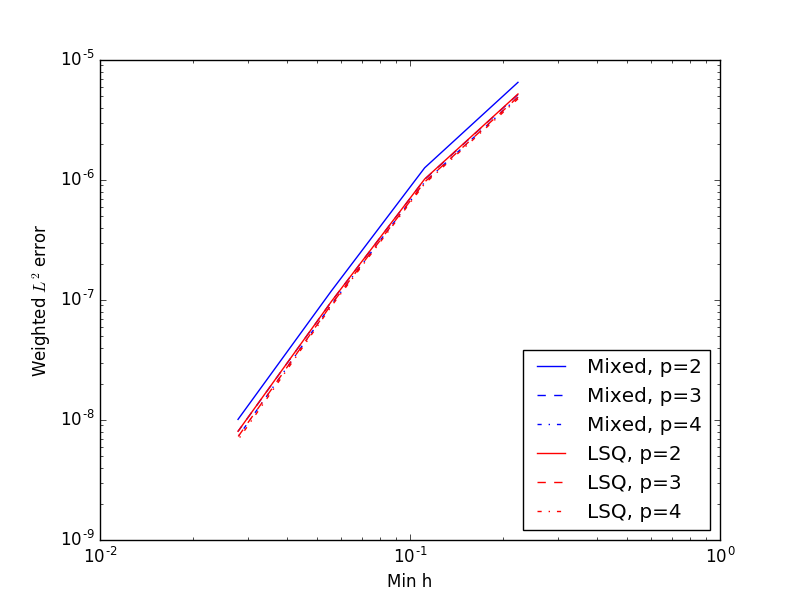
\includegraphics[width=0.85 \linewidth]{errs.PNG}
\caption{Change in nature of solution as $\alpha$ varies. Left to right: $\alpha =$ 0.5, -0.5, -1.}
\end{figure}

\newpage

\section*{Conclusion}
The Poisson problem was solved on a L-shaped domain. An analytical function was used to determine the behavior of the numerical error in the direct neighborhood to the elbow of the domain. It was found that LSQ finite element methods with h-refinement were the most efficient approach for convergence.

It should be noted that the preceding study optimizes for the very small region at the elbow of the domain. While this area presents the most numerical difficulties in terms of accuracy, it's effect on the overall domain is problem dependent. If local errors at the elbow are unimportant then these efficiency results may no longer hold true. However if the behavior at the elbow is important for the problem (e.g. crack propagation, fatigue lifetime estimation, etc.), then the results obtained will likely be a good choice.

\newpage

\begin{figure}[!htb]
\centering
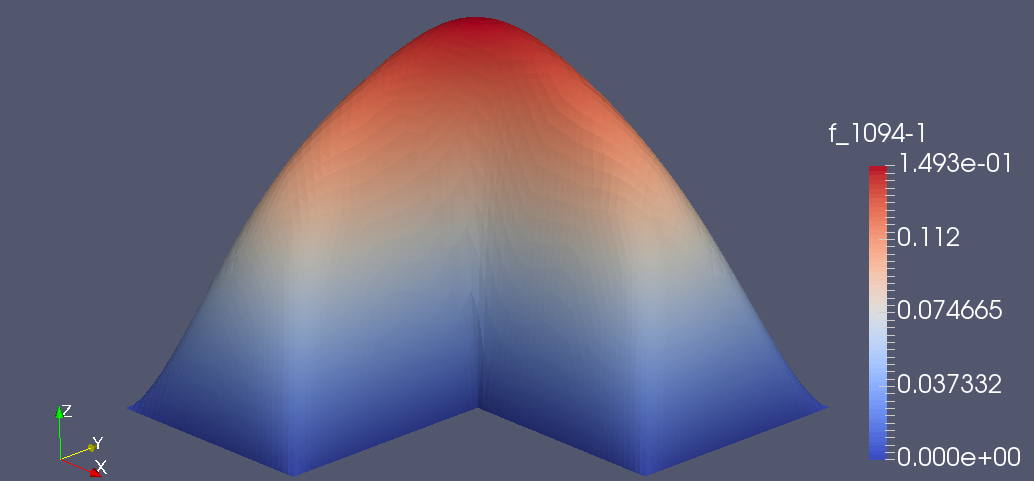
\includegraphics[width=1 \linewidth]{sol.PNG}
\caption{Observed behavior of convergence order as dependent on $\alpha$, quadratic elements.}
\end{figure}

\begin{figure}[!htb]
\centering
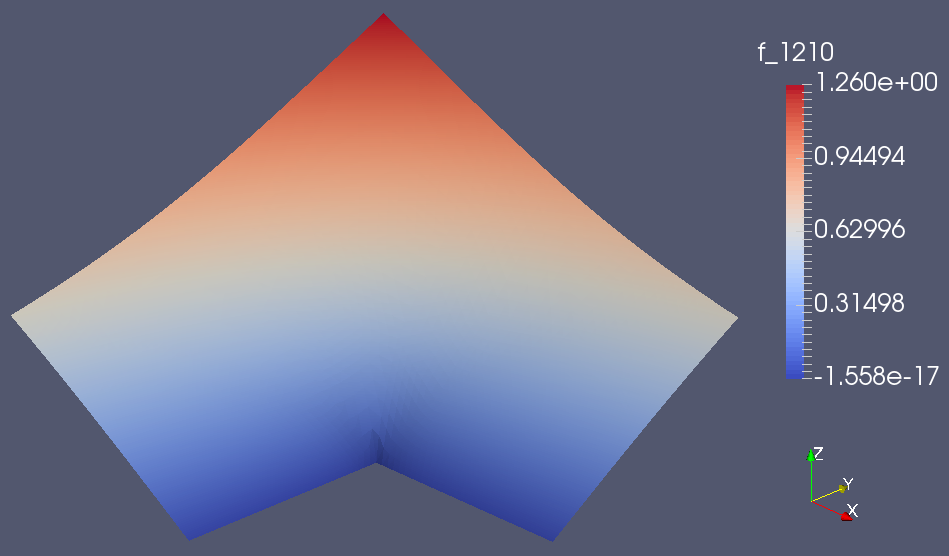
\includegraphics[width=1 \linewidth]{f.PNG}
\caption{Change in nature of solution as $\alpha$ varies. Left to right: $\alpha =$ 0.5, -0.5, -1.}
\end{figure}

\end{document}